Pogosto si moramo za rešitev različnih problemov podatke organizirati drugače,
kot da jih le shranimo v običajen seznam.
Z uvedbo posebnih \emph{podatkovnih struktur} lahko hitreje odgovarjamo na
različna vprašanja o shranjenih informacijah, kar lahko uporabimo kot sestavno
komponento v raznih algoritmih.
Poglejmo si primer.
Recimo, da imamo dan seznam števil dolžine $n$, nato pa bi radi $q$-krat
ugotovili, če je neko število v teh seznamu.

\fkoda{poglavja/podatkovne-strukture/primer-slabo.cpp}

Če si podatke le shranimo v seznam, kot zgoraj, potem bomo v najslabšem primeru
za vsako od poizvedb morali preiskati celoten seznam, torej je naša rešitev
$O(nq)$.
Za hitrejšo rešitev bi lahko seznam na začetku uredili, nato pa pojavitve števil
$k$ iskali z bisekcijo:

\fkoda{poglavja/podatkovne-strukture/primer-bisekcija.cpp}

Takšna rešitev ima časovno zahtevnost $O((n + q) \log n)$, saj za urejanje
porabimo $O(n \log n)$ časa, vsaka izmed $q$ poizvedb pa se izvede v $O(\log n)$
korakih.
Povedano drugače smo v zgornjem primeru opazili naslednje dejstvo:
Operacija \enquote{preveri, ali se dan podatek nahaja v podatkovni strukturi}
ima zahtevnost $O(n)$ v sezamu in $O(\log n)$ v urejenem seznamu.
Kaj pa lahko povemo o drugih operacijah, ki bi si jih želeli uporabljati v
algoritmih?

V nadaljevanju bomo za različne podatkovne strukture obravnavali časovno
zahtevnost naslednjih operacij:
\begin{enumerate}
\item[(O1)] dodaj podatek v podatkovno strukturo,
\item[(O2)] odstrani podatek iz podatkovne strukture,
\item[(O3)] preveri, če je podatek v podatkovni strukturi.
\end{enumerate}
Število podatkov, shranjenih v podatkovni strukturi, bomo označili z $n$.

\naslov{Seznami}

Najbolj osnovna podatkovna struktura je običajen seznam.
V računalniškem spominu je predstavljen z enim velikih blokom spomina, ki si ga
lahko predstavljamo kot $n$ spremenljivk istega tipa, položenih eno za drugo.
Ko deklariramo seznam, moramo nujno podati njegovo dolžino, da lahko prevajalnik
rezervira blok primerne velikosti.
Kakor smo povedali v uvodnem razdelku poglavja, za operacijo (O3) potrebujemo
$O(n)$ časa.
Pri določanju časovne zahtevnosti za operaciji (O1) in (O2) pa naletimo na
težavo.
Seznami namreč ne podpirajo dodajanja ali odstranjevanja podatkov --- število
elementov seznama je fiksno in določeno v kodi.
Lahko pa se pretvarjamo, da seznam podpira ti operaciji tako, da si zapomnimo
trenutno število podatkov v seznamu:

\fkoda{poglavja/podatkovne-strukture/seznam-simulacija.cpp}

Iz zgornje kode je jasno razvidno, da imata tako operaciji (O2) kot (O3) časovno
zahtevnost $O(n)$, saj moramo pri obeh v najslabšem primeru premakniti vse
elemente.
Opazimo pa lahko tudi, da potrebujeta operaciji \enquote{dodaj na konec seznama}
in \enquote{odstrani iz konca seznama} le konstantno mnogo časa, saj se v obeh
primerih zanka takoj konča.
To bo pomembno kasneje.

Druga težava z zgornjo implementacijo pa je ta, da naš seznam lahko shrani
največ $1000$ elementov.
Seveda bi lahko pri deklaraciji \koda{int arr[1000]} le povečali številko tako,
da bi bila dovolj velika za naše potrebe, vendar tega včasih ne želimo narediti
(na primer če imamo veliko majhnih seznamov in nekaj velikih, a ne vemo v
naprej, kateri od teh seznamov bodo velikih).
Lahko bi si namesto fiksnega seznama \koda{arr} hranili kazalec na del spomina,
kjer je seznam shranjen, ter širino tega dela spomina, ter ga po potrebi
povečali, kot spodaj:

\fkoda{poglavja/podatkovne-strukture/seznam-simulacija-malloc.cpp}

Funkcija \koda{odstrani_element} je v tem primeru enaka kot prej.
Napisali smo \emph{dinamični seznam}, tj.~seznam, ki prilagaja svojo hitrost
glede na število shranjenih elementov.
S tem pa smo izgubili zgoraj omenjeno lastnost, da je dodajanje na oz.~brisanje
iz konca seznama $O(1)$, saj bo tekom zgornjega programa velikost vedno enaka
kapaciteti, zato se bo prvi pogojni stavek v funkciji vedno aktiviral.
To lastnost pa lahko še vedno v neki obliki obdržimo, če naredimo majhno
spremembo:

\fkoda{poglavja/podatkovne-strukture/seznam-simulacija-konstantno.cpp}

Ko \koda{arr} povečamo, torej njegovo kapaciteto podvojimo.
Kaj pa smo s tem dejansko dosegli?
Ko v seznam dodamo prvi element, ne potrebujemo ničesar kopirati.
Ko dodamo drugi element, moramo prekopirati prvega.
Ko dodamo tretji element, moramo prekopirati prvega in drugega.
Pri četrtem elementu pa nam ni treba ničesar kopirati, saj je \koda{arr} že
dovolj velik, da lahko četrti element takoj shranimo vanj.
Za peti dodan element bomo morali spet prekopirati prve štiri, za šesti, sedmi
in osmi element pa nam ne bo treba ničesar kopirati.
Zapišimo še nekaj členov tega zaporedja (koliko elementov moramo prekopirati, ko
dodamo nov element v seznam):
\[
  0, 1, 2, 0, 4, 0, 0, 0, 8, 0, 0, 0, 0, 0, 0, 0, 16, \ldots
\]
Z nekaj razmisleka vidimo, da je vsota prvih $n$ členov tega zaporedja enaka
$2n$, če je $n$ ravno potenca števila $2$, oziroma $n$ v vseh ostalih primerih.
V povprečju bomo torej za dodajanje enega elementa na konec seznama porabili le
$O(1)$ časa.
Pravimo, da je ta operacija \emph{asimptotično konstantna} --- v povprečju
potrebujemo konstanten čas, da jo izvedemo, vsake toliko pa bo operacija trajala
dlje.

\podnaslov{Vektorji}

K sreči ne potrebujemo vsakič znova pisati svojih dinamičnih seznamov, saj so že
vključeni v standardni knjižnici C++ pod imenom \koda{vector}.
Poglejmo si, kako delujejo.

\fkoda{poglavja/podatkovne-strukture/vector.cpp}

Ko deklariramo vektor, v trikotnih oklepajih (znaka za manjše oz.~večje)
dopišemo še tip podatkov, ki jih bomo v vektor shranjevali.
V tem primeru uporabimo kar \koda{int}, lahko pa bi uporabili kakršenkoli drugi
tip, na primer \koda{char}, \koda{long long*}, \koda{vector<vector<int>>} itd.
Potem nam je na voljo več metod, ki jih uporabimo tako, da napišemo ime metode
za imenom spremenljivke in piko:
\begin{itemize}
\item metoda \koda{size()} vrne trenutno velikost vektorja,
\item metoda \koda{push_back(x)} doda \koda{x} na konec vektorja v $O(1)$,
\item metoda \koda{begin()} vrne iterator na začetek vektorja,
\item metoda \koda{end()} vrne iterator tik čez konec vektorja,
\item metoda \koda{insert(it, x)} doda \koda{x} tik pred mesto \koda{it} v
  $O(n)$,
\item metoda \koda{erase(it)} izbriše element na mestu \koda{it} v $O(n)$,
\item metoda \koda{clear()} izbriše vse elemente vektorja.
\end{itemize}
\emph{Iterator} je poseben tip podatkov, ki si ga lahko predstavljamo kot
kazalec (ker tudi podpira običajne operacije kazalcev).
Iterator dobimo iz metod \koda{begin()} in \koda{end()}, moramo pa ga podati kot
argument metodama \koda{insert()} in \koda{erase()}.
Iteratorjem lahko prištevamo številke, s čimer lahko dostopamo do poljubnega
elementa vektorja (ali pa to naredimo tudi z oglatimi oklepaji).

\podnaslov{Skladi}

Sklad je podatkovna struktura, ki podpira le dve operaciji:
\enquote{dodaj element na vrh sklada} in \enquote{odvzemi element z vrha
  sklada}.
Predstavljamo si, da elemente zlagamo na kup, iz katerega lahko jemljemo le
vrhnji element, ker bi se kup sicer prevrnil.

\fkoda{poglavja/podatkovne-strukture/sklad.cpp}

Poleg metod \koda{push()} in \koda{pop()} za dodajanje oz.~odstranjevanje
elementov imamo na voljo tudi metodi \koda{top()}, ki pogleda, kaj je shranjeno
na vrhu sklada, in \koda{size()}, ki vrne število elementov na skladu.
Vse metode imajo časovno zahtevnost $O(1)$.

Poglejmo si primer naloge, kjer v rešitvi uporabimo sklad.
Zadan nam je naslednji problem:
Dan je seznam števil, ki opisuje višino stolpnic, postavljenih v vrsto ena za
drugo.
Za vsako stolpnico ugotovi, katera je njej najbližja stolpnica na levi, ki je
višja od nje.
Za tretjo stolpnico na spodnji sliki je to stolpnica številka $2$, za četrto
stolpnico pa je odgovor enak $1$, saj sta stolpnici $2$ in $3$ nižji od
stolpnice $4$.

\begin{figure*}[h!]
  \centering
  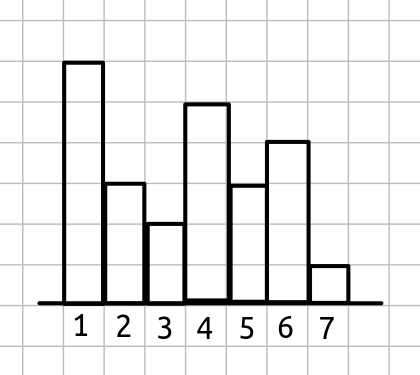
\includegraphics[width=0.5\linewidth]{poglavja/podatkovne-strukture/stolpnice}
\end{figure*}

\fkoda{poglavja/podatkovne-strukture/stolpnice.cpp}

Zgornji program bo rešil dan problem na očiten način v $O(n^2)$.
Obstaja pa tudi linearna rešitev, ki se poslužuje dveh skladov.
Osnovna ideja je, da si hranimo padajoče zaporedje stolpnic, ki so kandidati za
najbližjo višjo stolpnico na levi.
Ko pridemo do stolpnice, ki je nižja od najnižjega kandidata, lahko za njo takoj
zatrdimo, da je najnižji kandidat ravno iskani odgovor.
Če pa je najnižji kandidat višji od stolpnice, ki jo trenutno obravnavamo, vemo,
da ne bo ta kandidat nikoli več najbližja višja stolpnica, saj je trenutna
stolpnica hkrati višja od kandidata in bližje preostalim stolpnicam.
Torej lahko kandidate, ki so nižji od trenutne stolpnice, kar odstranimo iz
sklada.

V rešitvi imamo dve gnezdeni zanki (\koda{while} znotraj \koda{for}).
Zakaj je potem še vedno linearna?
Enostaven argument je, da bomo vsako stolpnico enkrat dodali v sklad, in jo
zato največ enkrat odstranili iz sklada, torej bomo v najslabšem primeru
opravili $2n$ operacij na skladu.

\fkoda{poglavja/podatkovne-strukture/stolpnice-linearno.cpp}

% \podnaslov{Vrste}

% \naslov{Množice}

% \podnaslov{Slovarji}

% \naslov{Prioritetne vrste}